%%% Thesis Introduction --------------------------------------------------
\chapter{REVIEW OF LITERATURE}
%%% ----------------------------------------------------------------------
\indent\indent\indent  Mechanics is the branch of mathematics which deals with matter in motion or at rest. Fluid is a substance which deforms continuously without any limit as long as we apply stress on it. Fluid mechanics is define as the subdivision of mathematics which deals with fluid in motion or at rest. It covers a vast spectrum of topics such as turbines, magnetohydrodynamic, air flight, pipe networks and biomedical applications etc.\\
 %\noindent Fluid mechanics is divided into fluid statics, fluid kinematics and fluid dynamics. Fluid statics is the branch of fluid mechanics which deals with the fluids at rest. Fluid kinematics is the branch of fluid mechanics in which we study the fluid in motion without considering the forces that affects the motion. Fluid dynamics is the branch of fluid mechanics in which we discuss the fluids in motion with considering forces that affects the motion. \\
 %\noindent Fluid statics which is also called hydrostatics is basic to
  %applied science engineering of machinery for storing, transporting and using fluids.\\
 %\noindent Fluid dynamics has a wide range of applications including determining the mass flow rate of petroleum through pipelines, understanding nebulae in interstellar and in crowd dynamics. It is also used in traffic engineering as road geometry, traffic lights, side walks and traffic signs.\\
 \noindent Fluid is further divided into two fluids.
 \begin{enumerate}
   \item \textbf{ Newtonian fluid} is defined as the fluid whose viscosity remains constant as the force applied changes. For a Newtonian fluid, the proportionality constant being the coefficient of viscosity. No real fluid fits the description but for simplicity of solving the problems in ordinary conditions we consider air and water as Newtonian fluids.
   \item  \textbf{Non-Newtonian fluid} is defined as a fluid whose viscosity changes depending on the applied force.  Non-Newtonian fluids are of three types:\begin{description}
               \item[
              (i) Shear thinning fluid or Pseudo-plastic]  are the fluids whose viscosity decreases with applied stress\ e.g\ \  blood, lipstick, polymeric solutions.
               \item[(ii) Shear thickening or
               Dilatant]  are the fluids whose viscosity increases with applied stress\ e.g \ \ butter, water starch mixture, quick sand.
               \item[(iii) Bingham plastics]  are the materials which behaves as solid at low stress and as fluid at high stress\ e.g \ \ tooth paste, mayonnaise.
             \end{description}
 \end{enumerate}

\noindent The root of the  historical development of fluid mechanics is due to the contributions of many mathematicians, engineers and scientists. A Greek mathematician Archimedes(287 BC-212 BC) constructed the laws of buoyancy and applied these laws to immerse bodies. Sailing ships and irrigation systems are the applications of his law.
\begin{figure}\begin{center}
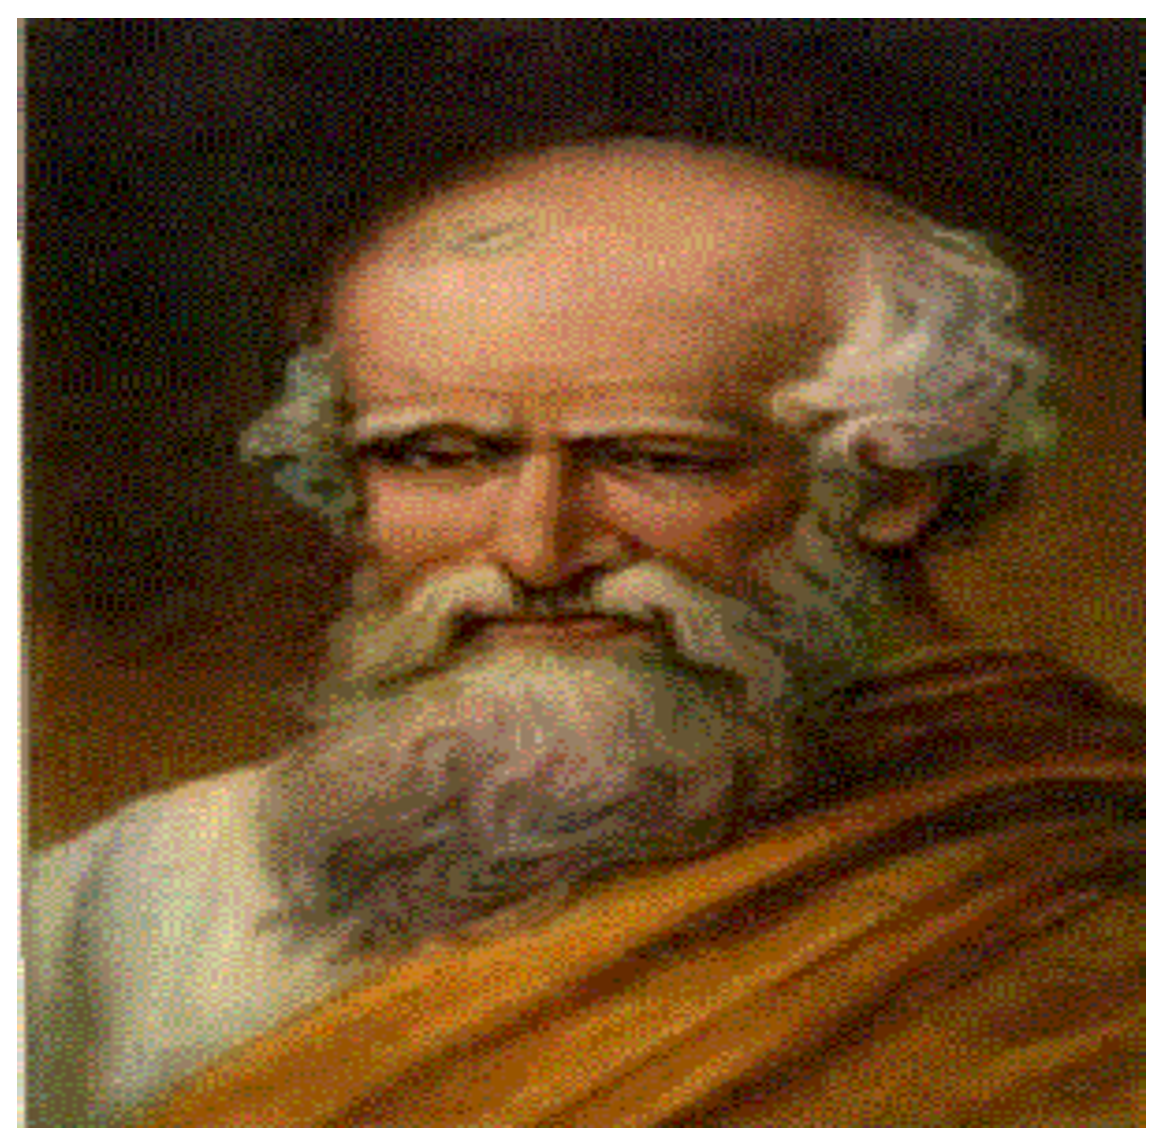
\includegraphics[width=6cm, height=6cm]{archimedes.eps}
\caption{Archimedes }\label{fig:Archimedes}
\end{center}\end{figure}

 Then Leonardo da Vinci (1452-1519) presented an idea of equation of motion  in one dimension. Evangelista Torricelli (1608-1647) formulated a  mercurial barometer, this was the first barometer.\\
 \indent For the necessary betterment in the study of fluid flow, a Frenchman Edme Mariotte (1620-1684) did work  on the air gases along with the  establishment of the underground wind canal.
Blaise Pascal (1623-1662) inventions include the hydraulic press as well as he does alot of work to study fluids. He clear the ideas of pressure and space. Isaac Newton (1642-1727) formulated laws of motion along with law of viscosity of the linear fluids.
\begin{figure}\begin{center}
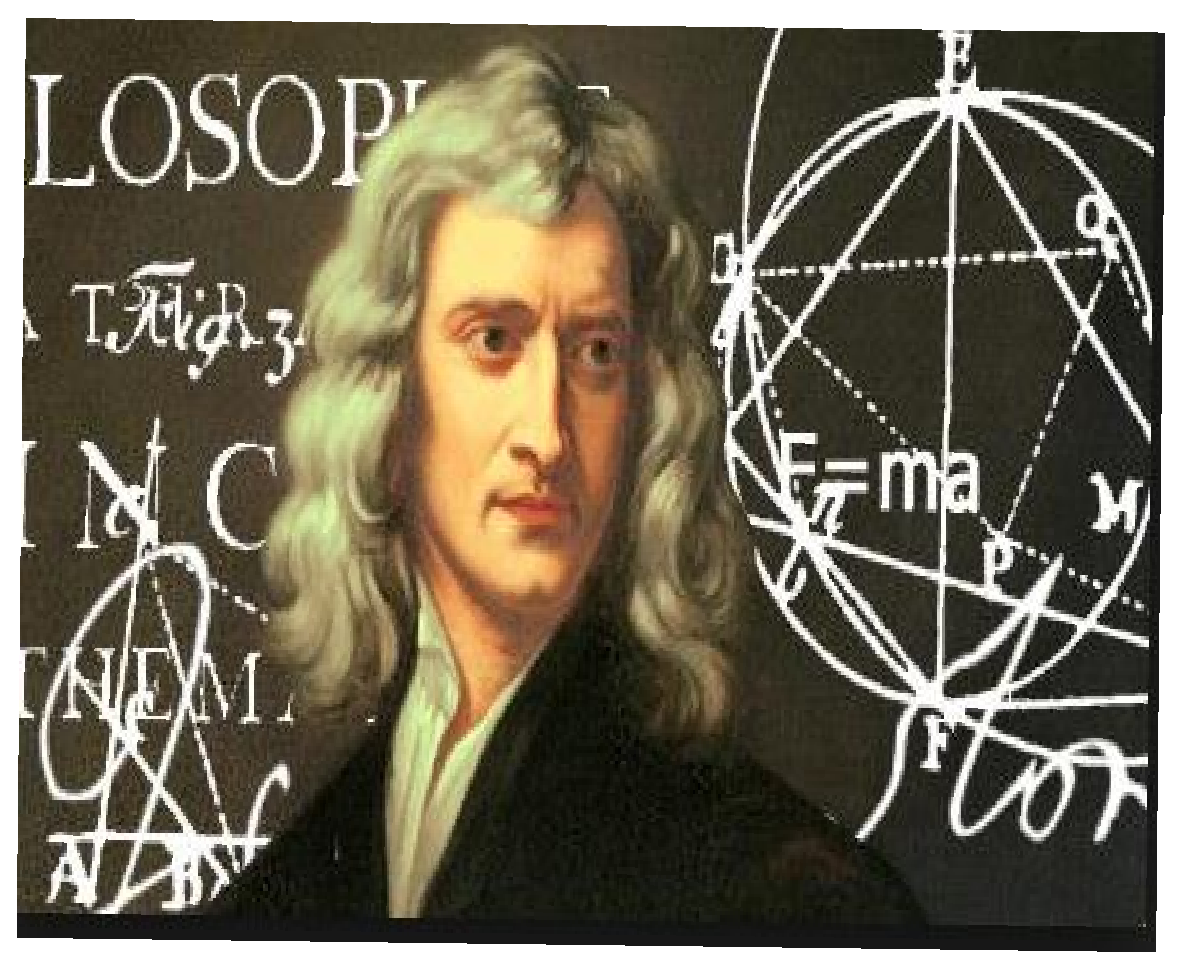
\includegraphics[width=6cm, height=6cm]{newton.eps}
\caption{Issac Newton }\label{fig:Isaac Newton}
\end{center}\end{figure}


dfdskfjsdljkfjs


\begin{table}
	\centering
	\renewcommand{\arraystretch}{1.5}
	\begin{tabular}{|c|c|c|c|c|c|c|c|c|c|c|}
		\hline
		% after \\: \hline or \cline{col1-col2} \cline{col3-col4} ...
		$ K_I$ & $\lambda$ & $\delta_m$ & $\sigma$ & M & $N_t$ & $N_b$ & Sc & Pr & $\gamma$ & -$\varphi$'($\eta$) \\ \hline
		0.11 & 0.11 & 0.51 & 0.51 & 0.11 & 0.11 & 0.31 & 11 & 11 & 0.11 & 0.5615 \\
		0.31 & 0.11 & 0.51 & 0.51 & 0.11 & 0.11 & 0.31 & 11 & 11 & 0.11 & 0.5441 \\
		0.51 & 0.11 & 0.51 & 0.51 & 0.11 & 0.11 & 0.31 & 11 & 11 & 0.11 & 0.5363 \\
		0.11 & 0.11 & 0.01 & 0.51 & 0.11 & 0.11 & 0.31 & 11 & 11 & 0.11 & 0.5647 \\
		0.11 & 0.11 & 0.31 & 0.51 & 0.11 & 0.11 & 0.31 & 11 & 11 & 0.11 & 0.5584 \\
		0.11 & 0.11 & 0.71 & 0.51 & 0.11 & 0.11 & 0.31 & 11 & 11 & 0.11 & 0.5470 \\
		0.11 & 0.11 & 0.11 & 0.01 & 0.11 & 0.11 & 0.31 & 11 & 11 & 0.11 & 0.6094 \\
		0.11 & 0.11 & 0.51 & 0.11 & 0.11 & 0.11 & 0.31 & 11 & 11 & 0.11 & 0.5635 \\
		0.11 & 0.11 & 0.51 & 0.21 & 0.11 & 0.11 & 0.31 & 11 & 11 & 0.11 & 0.5343 \\
		0.11 & 0.11 & 0.51 & 0.51 & 0.01 & 0.11 & 0.31 & 11 & 11 & 0.11 & 0.5441 \\
		0.11 & 0.11 & 0.51 & 0.51 & 0.21 & 0.11 & 0.31 & 11 & 11 & 0.11 & 0.5222 \\
		0.11 & 0.11 & 0.51 & 0.51 & 0.41 & 0.11 & 0.31 & 11 & 11 & 0.11 & 0.4939 \\
		0.11 & 0.11 & 0.51 & 0.51 & 0.11 & 0.11 & 0.31 & 21 & 11 & 0.11 & 0.8402 \\
		0.11 & 0.11 & 0.51 & 0.51 & 0.11 & 0.11 & 0.31 & 31 & 11 & 0.11 & 1.0651 \\
		0.11 & 0.11 & 0.51 & 0.51 & 0.11 & 0.11 & 0.21 & 41 & 11 & 0.11 & 1.2557 \\
		0.11 & 0.11 & 0.51 & 0.51 & 0.11 & 0.11 & 0.31 & 11 & 11 & 0.21 & 0.6942 \\
		0.11 & 0.11 & 0.51 & 0.51 & 0.11 & 0.11 & 0.31 & 11 & 11 & 0.41 & 0.8348 \\
		0.11 & 0.11 & 0.51 & 0.51 & 0.11 & 0.11 & 0.31 & 11 & 11 & 0.61 & 0.9526 \\
		\hline
	\end{tabular}\\
	\caption{The numerical local Sherwood number values for the parameters involved}
	\label{table:2}
\end{table}








